\section{Robustness Interfaces and Certificate Verification}
\label{sec:verification}

\subsection{Loewner proxy robustness}

\begin{proposition}[Proxy inflation]
\label{prop:proxy-inflation}
If
\[
  (1-\varepsilon)H\preceq\widehat H\preceq(1+\varepsilon)H,
  \qquad 0\le\varepsilon<1,
\]
then every \(G\succ0\) satisfies
\[
  \kappa(G^{-1}H)
  \le
  \frac{1+\varepsilon}{1-\varepsilon}
  \kappa(G^{-1}\widehat H).
\]
Consequently, reaching the proxy threshold
\[
  \widehat K=K\frac{1-\varepsilon}{1+\varepsilon}
\]
is sufficient for the true threshold whenever \(\widehat K\ge1\).
\end{proposition}

\begin{proposition}[High-probability proxy interface]
\label{prop:stoch-proxy-upper}
Suppose a random proxy obeys the displayed Loewner event with probability at
least \(1-\delta\).  If a structured candidate \(G\) satisfies
\(\kappa(G^{-1}\widehat H)\le\widehat K\) on that event, then
\(\kappa(G^{-1}H)\le K\) with probability at least \(1-\delta\).
\end{proposition}

The second statement is an interface.  A finite-sample result requires a
concentration theorem for the chosen estimator \cite{tropp2015matrix}.

\subsection{Deterministic and randomized checks}

The accompanying code supplement contains deterministic and randomized
small-SPD checks for diagonal and block certificates, Kronecker spectral
mismatch, Hessian-relative candidates, projection residuals, and strict
separation.  The entry points are
\begin{itemize}[leftmargin=*,itemsep=0em,topsep=0.2em]
  \item \texttt{synthetic\_certificate\_benchmark.py},
  \item \texttt{random\_spd\_certificate\_suite.py},
  \item \texttt{kron\_certify\_demo.py}.
\end{itemize}
Failed identities raise assertions.  The
reference environment is Python 3.11.4 with NumPy 1.26.4, SciPy 1.10.1,
Matplotlib 3.7.1, and SymPy 1.11.1.

In the randomized suite, seeds \(0,\ldots,63\) are used.  The diagonal target
\(K=3\) is reachable in 32 instances, the block-Jacobi target \(K=3\) is
certified in 58, and the fixed-basis Kronecker spectral target \(K=3\) is
reachable in 57.  All 64 constructed Hessian-relative Kronecker positive
controls reach \(K=2\), while the identity constructed negative control fails
that target in all 64 cases.

The positive controls use
\[
  H=G^{1/2}CG^{1/2},
  \qquad
  \kappa(C)\in[1.1,1.8],
\]
with target \(K=2\).  The counts therefore measure theorem-check coverage in
the declared suite, not population success probabilities.

For an independent projection check, the noncommuting \(2\times2\) example is
also optimized by generic BFGS in a five-dimensional gauge-fixed log-factor
chart.  Three deterministic starts agree on the objective to less than
\(2\times10^{-15}\).  The partial-trace Armijo iterate stops at residual
\(8.257\times10^{-6}\); its objective exceeds the independent value by
\(3.227\times10^{-11}\), below the theorem's residual bound
\(3.409\times10^{-11}\), and the two matrices are AIRM distance
\(7.823\times10^{-6}\) apart.  BFGS uses gradient tolerance \(10^{-7}\);
Armijo uses initial step one, shrink factor \(1/2\), parameter \(10^{-4}\),
and residual tolerance \(10^{-4}\).  These calculations test the theorem
through a distinct parameterization and optimizer; they do not establish a
large-scale complexity claim.

The same deterministic script directly checks the marginal criterion in
\cref{thm:kron-nearest-versus-best,cor:kron-marginal-mismatch,%
cor:kron-two-by-two-completeness}.  For the exact \(2\times3\) separation,
the projection normal residual is zero and
\(\mu_{\mathrm{marg}}=0.816496580927726\).  Hence the predicted one-sided
descent slope is \(-\mu_{\mathrm{marg}}^2=-2/3\); a step of \(10^{-6}\)
gives the finite-difference slope \(-0.666666666759852\).  In a deterministic
\(2\times2\) Bell-canonical instance with projection log-condition \(2.2\),
the projection normal residual is zero and the computed marginal mismatch is
\(3.21\times10^{-16}\).  These two checks exercise respectively the strict
separation and the low-dimensional completeness mechanisms.

The deterministic sensitivity scan varies the diagonal coupling and target
\(K\), block coupling, fixed-basis Kronecker threshold, and low-rank spectral
budget.  It contains 86 finite and 49 unreachable diagonal grid entries; the
maximum block primal and dual numerical violations are
\(2.21\times10^{-16}\) and zero.  The low-rank reachable threshold decreases
monotonically from \(121.51\) at rank zero to \(1\) at full rank, as required
by \cref{prop:lowrank-monotonicity}.  These parameter scans expose certificate
branch changes and numerical residuals rather than estimating a data-generating
success probability.

\begin{figure}[htbp]
  \centering
  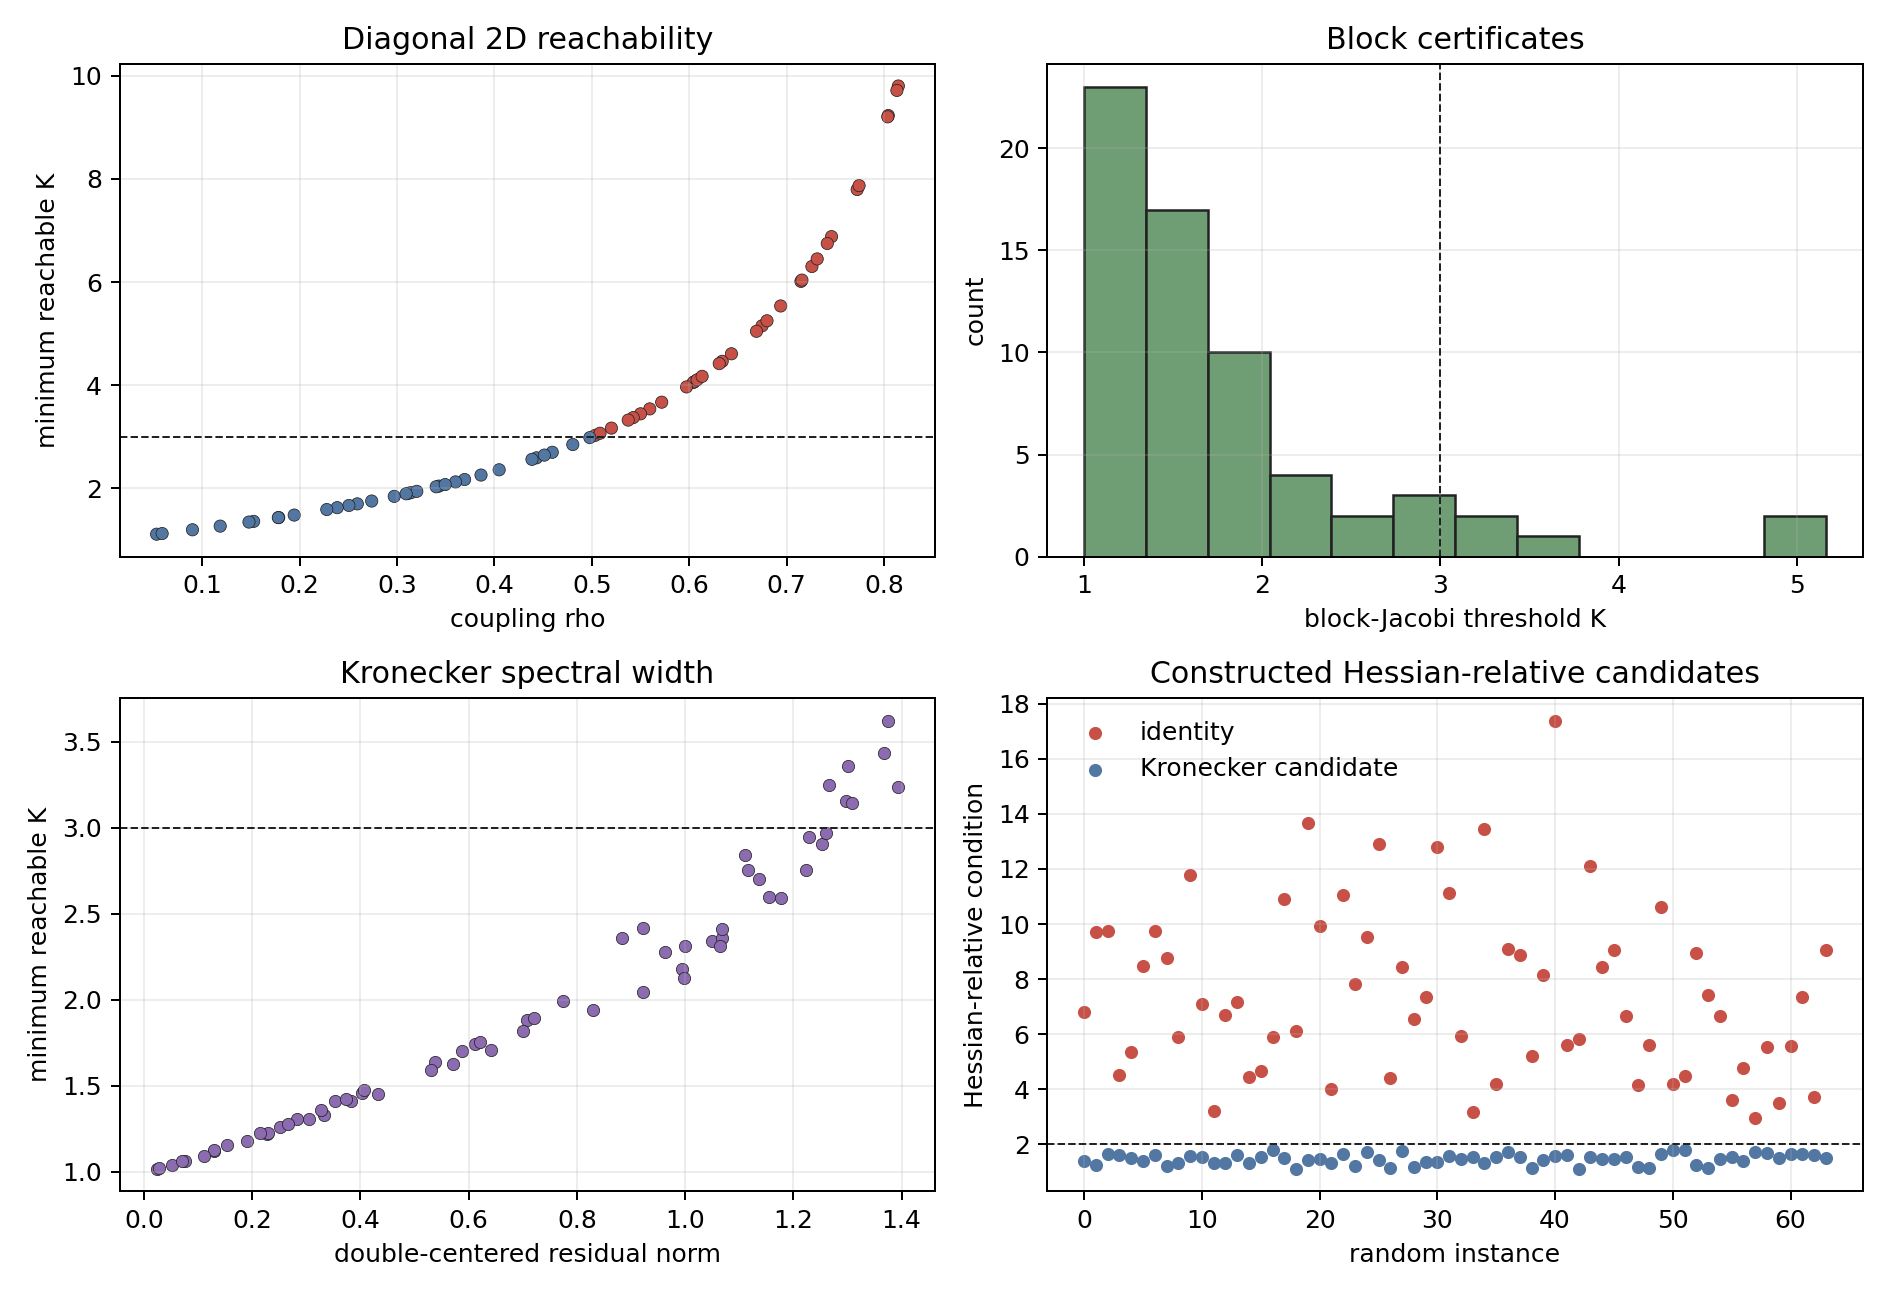
\includegraphics[width=\linewidth]{figures/random_spd_certificate_suite.png}
  \caption{Randomized small-SPD certificate checks over 64 seeds.  The panels
  record diagonal reachability, block-Jacobi thresholds, fixed-basis
  Kronecker spectral width, and constructed Hessian-relative Kronecker
  candidates.  The identity is a constructed negative control.  These are
  theorem checks, not optimizer comparisons.}
  \label{fig:random-spd-suite}
\end{figure}

\FloatBarrier
